Non benissimo i link nel sito, che soffrono dei seguenti problemi:
\begin{itemize}
	\item \textbf{Colore} : quando un link è già stato visitato dovrebbe cambiare colore in modo che l'utente non debba tenersi a mente la pagine già visualizzate. Questo non accade nel sito, dove tutti i link sono neri o grigi. Sarebbe stato quantomeno possibile colorare quelli già visitati di un grigio più chiaro.
	\item \textbf{Disomogeneità} : Molti link, anche con funzioni simili, sono graficamente diversi. Alcuni hanno una freccetta vicina, altri cambiano colore quando ci si passa sopra, altri ancora sono sottolineati.
	\item \textbf{Entra in} : molti link sono posti sotto blocchi di testo, e sono nella forma "Entra nel dettaglio X". In molti casi sarebbe stato possibile rendere cliccabile direttamente il titolo del paragrafo.
\end{itemize}

\begin{figure}[H]
	\centering
	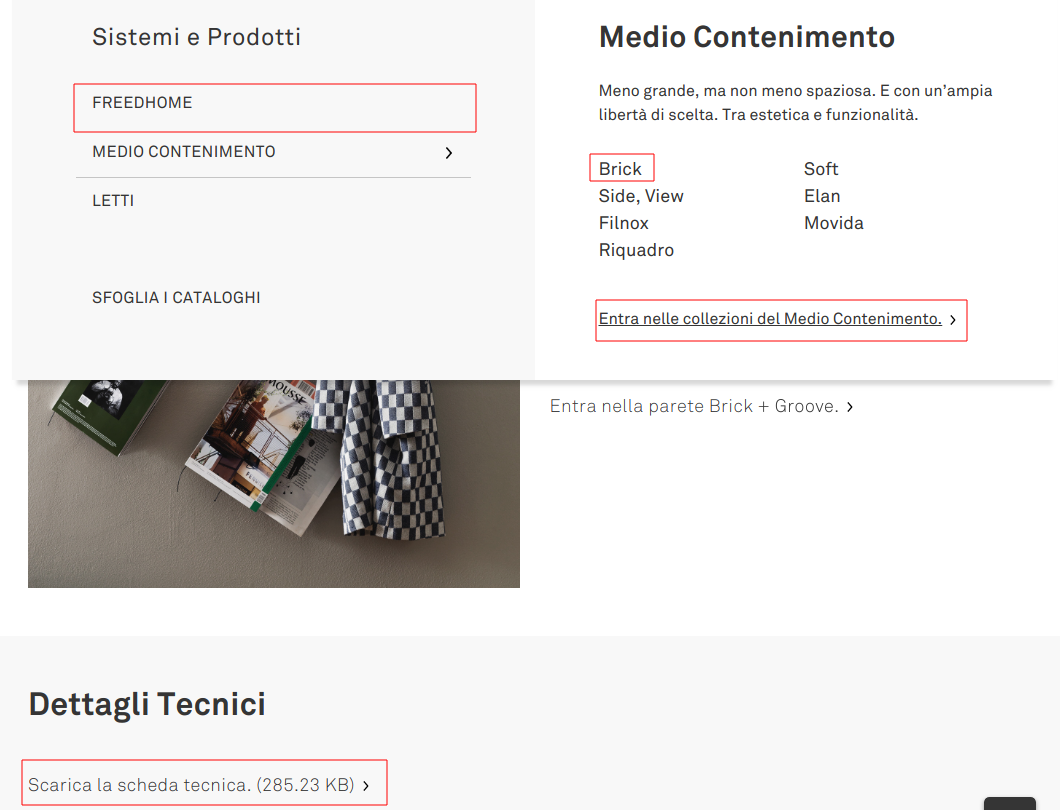
\includegraphics[width=\textwidth ,keepaspectratio]{sez/Elementi_Comuni/img/link.png}
	\caption{4 esempi di link cliccabili in una sola schermata: nessuno cambia colore se già visitato.}
\end{figure}

\begin{center}
\begin{Large}
\textbf{VOTO}\\
\vspace{0.1cm}
\end{Large}
\begin{huge}
5+
\end{huge}
\end{center}